\chapter{Stochastic programming}
\label{chap1}

%
%Structure of thesis:
%Introduction
%Multistage stochastic programming problems
%-multistage idea, nonanticipativity constraints, deterministic equivalent
%-curse of dimensionality
%-scenario trees
%    -moment matching, geometric brownian motion + clustering (glasserman 2003, Andrej Uhliarik thesis)
%Risk measures
%-VaR, CVaR, minimisation, L shaped method, reformulating as a multistage program
%Reinforcement learning
%-introduction, comparison to other types (supervised etc), no loss function - inspiration from learning of animals and men
%-Basic idea
%-Multiarmed bandits
%Study
%-Formulation of the whole problem (idea of thesis)
%-Related work e.g. Galuzzi, B.G., Messina, E., Candelieri, A., Archetti, F. (2020). Optimal Scenario-Tree %Selection for Multistage Stochastic Programming. In: , et al. Machine Learning, Optimization, and Data Science. %LOD 2020. Lecture Notes in Computer Science(), vol 12565. Springer, Cham. https://doi.org/%10.1007/978-3-030-64583-0_31
%    -Idea how to evaluate
%    -Penalisation of result using complexity of tree with a hyperparameter - explain reasoning why we should penalise the result - why are complex scenario trees bad (long computation time, ...)?
%-Data
%-Computational problems, complexity, how long does solving each small problem take
%-Results of the study
%

%Stochastic programming
%-Framework to model problems which involve uncertainty
%-Optimization problem where some or all parameters are uncertain in contrast to deterministic optimization
%-the goal is to find a solution which is feasible for all such data and optimal in some sense
%-Stochastic programming models are similar in style but take advantage of the fact that probability distributions governing the data are known or can be estimated
%-The goal is to find some policy that is feasible for all (or almost all) the possible parameter realizations
%and optimizes the expectation of some function of the decisions and the random variables
%-Areas where stochastic programming is used
%	-financial planning, airline scheduling, transportation (truck routes, daily milk delivery with random demand), management of power systems

In this chapter, we give an introduction to the theory of stochastic programming with particular focus on multistage linear programs. Most of the content in this chapter is based on the material covered in \cite[Chapter 1]{stochasticprogrammingbible}, \cite[Chapters 1-3]{stochasticprogrammingbible2009} and \cite[Part 2]{dupacovastochasticprogramming} if not specified otherwise.
\todo{Add more meat here}

\section{Basic definitions}
\begin{defn}{Mathematical program in $\R^n$ \cite[p. 107]{dupacovastochasticprogramming}}. \\
\label{def:MathematicalProgramDef}
Let $p,m,n \in \N$. A mathematical program in $\R^n$ is defined as
\begin{equation*}
\mathrm{min} \{f(\mathbf{x}), \mathbf{x} \in \mathbf{M}\},
\end{equation*}
where $\mathbf{M} \subset \R^n$ and $f$ is a real function. The function $f$ is called the objective function and the set $\mathbf{M}$ is called the set of feasible solutions.
This set is usually defined by constraints as follows:
\begin{equation*}
	\mathbf{M} = \{\mathbf{x} \in \R^n: h_j(\mathbf{x})=0, \, j=1,\dots,p, \, g_k(\mathbf{x}) \leq 0, k=1,\dots,m \},
\end{equation*}
where $h_j$ and $g_k$ are real functions.
\end{defn}
If all functions in Definition~\ref{def:MathematicalProgramDef} are linear, we call the problem a \textit{Linear program}.
Furthermore, if any of the functions mentioned in Definition~\ref{def:MathematicalProgramDef} depend on parameters, we call the problem a \textit{Parametric program}. If any of the parameters are uncertain \textcolor{red}{(random variables)}\todo{Is random variable ok here? I assume it is, just for check.}, we call the problem a \textit{Stochastic program}.


However, this definition of a Stochastic program is not well formulated. Consider the Definition~\ref{def:MathematicalProgramDef} and let $\Omega$ be a non-empty set, $\mathcal{F}$ be a  $\sigma$-algebra on $\Omega$, $\omega \in \Omega$ and $\mathcal{P}$ be a probability measure on $(\Omega, \mathcal{F})$, leading to a probability space $(\Omega, \mathcal{F}, \mathcal{P})$. In the context of a Stochastic program, the function $f$ does not depend on $\mathbf{x}$ only, but also on the realisation of $\omega$. This would lead to a nonsensical definition, as for different realisations of $\omega$, the optimal value may be different. The standard way to handle this problem is to consider minimisation of expected value of the function $f$:

\begin{equation*}
\mathrm{min} \{\mathbb{E}\left[f(\mathbf{x}, \omega)\right], \mathbf{x} \in \mathbf{M}\},
\end{equation*}
where $\mathbb{E}$ is the expected value operator defined with respect to the probability measure $\mathcal{P}$. \todo{Are these definitions (mostly the probability measure stuff) correct?}


\section{Multistage stochastic programming}
In the most basic form, the stochastic programming paradigm allows to make an optimal decision with regard to the expectation only for one decision period. This is a considerable limitation, which can be overcome by extending the notion of a \textit{Stochastic program} to a \textit{Multistage stochastic program}.

\subsection{Notation and general idea}
This section is heavily inspired by \cite[Section 3.3.]{stochasticprogrammingbible}.
Following the notation established there, consider the following sequence of events
\begin{equation*}
\begin{gathered}
\mathrm{Decision} \, \, x_1
\\
\downarrow
\\
\mathrm{Observation} \,\, \xi_2
\\
\downarrow
\\
\mathrm{Decision} \,\, x_2
\\
\downarrow
\\
\mathrm{Observation} \,\, \xi_3
\\
\downarrow
\\
\vdots
\\
\downarrow
\\
\mathrm{Observation} \,\, \xi_T
\\
\downarrow
\\
\mathrm{Decision} \,\, x_T,
\end{gathered}
\end{equation*}
where $T$ is the number of stages, $x=(x_1,\dots,x_T)$ is called the decision process ($x_1$ is a non-random vector of variables), $\xi = (\xi_2,\dots,\xi_{T})$ is a stochastic data process ($\xi_1$ is assumed to be known and deterministic). The decision process $x$ represents the decisions made at each stage (i.e. for a portfolio allocation problem, $x_t$ may be a random vector of proportions of some assets in a portfolio at some intermediate stage\todo{is this clear? Maybe rewrite}) and $\xi_{T}$ is a random vector representing the data proccess in the last stage (i.e. it may be a vector of yearly asset returns). Furthermore, the probability distribution of $\xi$ is assumed to be known.
\todo{make notation consistent regarding $\xi$}
\subsection{Nonanticipativity}
Both processes $x$ and $\xi$ are random and thus depend on the realised $\omega \in \Omega$. In order for the program to be well defined, the decision process $x$ must not take into account future observations of either
$\xi$ or decisions $x$, but only the past and present. This is formalised by the so called nonanticipativity constraints, which assure that the $x_t$ may depend only on $(x_1,\dots,x_{t-1})$ and $(\xi_1,...,\xi_{t})$.

\begin{defn}{Nonanticipativity constraints} \cite[Section 3.3.]{stochasticprogrammingbible}. \\
\label{def:nonanticipativity constraints}
The decision process $x$ is termed nonanticipative if
\begin{equation*}
x_t=\mathbb{E}\left[x_t|\xi_1,\dots,\xi_t \right], t=1,\dots,T,
\end{equation*}
or equivalently, if $\mathcal{F}_t$ is the $\sigma$-algebra generated by $(\xi_1,\dots,\xi_t)$, then $x_t(\omega)$\todo{should ($\omega$) be here?} must be measurable with respect to $\mathcal{F}_t$, where $\mathcal{F}_1 \subset \mathcal{F}_2 \subset \dots \subset \mathcal{F}_T \subset \mathcal{F}$.
\end{defn}
This is in contrast to general deterministic (multiperiod) programs, where all data are taken into account.

\subsection{General multistage optimization problem formulation}
\begin{defn}{Multistage nested problem formulation \cite[Section 3.1.1.]{stochasticprogrammingbible2009}} \\
Let $\xi=(\xi_1,\dots,\xi_{T})$ be the data process as defined in the previous sections, \\ $x=(x_1,\dots,x_t)$ the decision vector, $n_t$ and $d_t$ be the dimensions of $x_t$ and $\xi_t$ respectively, $f_t: \R^{n_t} \times \R^{d_t} \rightarrow \R$ be continuous functions and $
\mathcal{X}_t$ be the sets of constraints at each stage $t=1,\dots,T$. The general multistage optimization problem is then formulated as follows:
\footnotesize
\begin{equation}
\label{eq:generalmultistageprogrammingformulation}
\underset{x_1 \in \mathcal{X}_1}{\mathrm{min}}
 f_1(x_1) + \mathbb{E}\left[ \underset{x_2 \in \mathcal{X}_2(x_1, \xi_2)}{\mathrm{inf}} f_2(x_2,\xi_2) + \mathbb{E}\left[\dots + \mathbb{E}\left[ \underset{x_T \in \mathcal{X}_T(x_{T-1}, \xi_T)}{\mathrm{inf}} f_T(x_T,\xi_T)\right] \right] \right],
\end{equation}

\normalsize
where the sets $\mathcal{X}_t(x_{t-1},\xi_t)$ are random, since they dependend on $\xi_t$ and $x_{t-1}$, $t=2,\dots,T$.
\todo{Check this is all correct}
\end{defn}


\subsection{Linear programming formulation}
If the functions $f_t$ and constraints defining the sets $\mathcal{X}_t$, $t=1,\dots,T$ are linear in Equation \ref{eq:generalmultistageprogrammingformulation}, then we say that the problem is a \textit{Multistage linear programming problem}.

\begin{defn}{Multistage nested linear problem formulation \cite[Ch. 1, p. 25]{stochasticprogrammingbible}}. \\
Let $f_1=c_1^Tx_1$, $\mathcal{X}_1=\{x:A_{1,1}x_1=b_1, x \geq 0 \}$, $f_t = {c_t}^tx_t$, $\mathcal{X}_t=\{x:A_{t,t-1}x_{t-1}+A_{t,t}x_t=b_t\, , x \geq 0\}$, $t=2,\dots,T$, where $A_{t,t}, A_{t,t-1}$ are matrices and $b_t, c_t$ are vectors of consistent dimensions. \todo{is this "matrices and vectors of consistent dimensions" enough or should I specify explicitly?} Assuming that all infima are attained and all expectations exist, rewriting Equation \ref{eq:generalmultistageprogrammingformulation}, we obtain:
\footnotesize
\begin{equation}
\label{eq:nestedlinearmultistageprogrammingformulation}
\underset{\underset{x_1 \geq 0}{A_{1,1}x_1=b_1}}{\mathrm{min}}
 c_1^Tx_1 + \mathbb{E}\left[ \underset{\underset{x_{2} \geq 0}{A_{2,1}x_{1}+A_{2,2}x_2=b_2}}{\mathrm{min}} {c_2}^Tx_2 + \mathbb{E}\left[\dots + \mathbb{E}\left[ \underset{\underset{x_{T} \geq 0}{A_{T,T-1}x_{T-1}+A_{T,T}x_T=b_T}}{\mathrm{min}} {c_T}^Tx_T\right] \right] \right],
\end{equation}
\normalsize
where the quantities $c_t, A_{t,t-1}, A_{t,t}, b_{t}$ are random, or according to notation established earlier, $\xi_t=(c_t, A_{t,t-1}, A_{t,t}, b_{t})$, $t=2,\dots,T$. \todo{should $t=2$ be here or $t=1$?}
\end{defn}

If we view the decision process $x_t$ (at time $t$) as a function of the part of the data process $\xi$ known up to time $t$, i.e. $x_t=x_t(\xi_1,\dots,\xi_t)$, we can properly rewrite the multistage linear programming problem (Equation \ref{eq:nestedlinearmultistageprogrammingformulation}) in the same general form as other linear programming problems:
\begin{defn}
{Multistage linear problem formulation. \\ \cite[Ch. 1, p. 22]{stochasticprogrammingbible}} \todo{is formatting of this definition ok? Particularly the citation.}\\
\footnotesize
\begin{alignat}{10}
\label{eq:staircaselinearprogrammingformulation}
& &&  && \underset{x_1 \geq 0, x_2,\dots,x_T \overset{a.s.}{\geq} 0}{\mathrm{min}}  &&  \mathbb{E}\left[ c_1^Tx_1 + \dots +  c_T^Tx_T \right] && \\
& s.t. \, && A_{1,1}x_1 && && && \,=b_1 \nonumber \\
& && A_{2,1}x_1 +  && A_{2,2}x_2 && && \overset{a.s.}{=}b_2 \nonumber \\
& && && A_{3,2}x_2  +  A_{3,3}x_3 && && \overset{a.s.}{=}b_3 \nonumber \\
& && && && && \vdots \nonumber \\
& && && && A_{T,T-1}x_{T-1}  +  A_{T,T}x_T  && \overset{a.s.}{=}b_T \nonumber
\end{alignat}
\normalsize
,
\end{defn}
where the nonanticipativity constraints are included implicitly.

All aforementioned stochastic programming problems may involve general distributions, which, in particular, may be continuous. The literature suggests that while formulating such multistage stochastic programs is possible, solving such programs is not feasible. Particularly \cite{pflugscenariotreegeneration} mentions that this is \textit{due to the fact that the decisions are functions, making the problem a functional optimization problem, which cannot be numerically solved as it is}. We need to keep in mind that the resulting formulation is only approximate and solving it thus provides an estimate of the true objective value (and true decision variables).
\subsubsection{Formulation using scenario trees}
To obtain a solvable program, we must obtain a suitable approximation of the underlying continuous distribution. This approximation may be a discrete distribution with a finite number of atoms (scenarios) $\xi^i, i=1,\dots,S$ where $S$ is the number of scenarios. The scenarios are usually organised in tree form as shown in Figures \ref{fig:balanced_scenario_tree} and \ref{fig:unbalanced_scenario_tree}. The following description of scenario tree formulation is heavily inspired by \cite[Section 2]{dupacova_scenarios_for_multistage_stochastic_programs}.

Consider a multistage program with $T$ stages. In each of these stages, we need to find a discretization of the underlying distribution, particularly the marginal distribution in the first stage and the conditional distributions in the intermediate stages. The number of atoms in each of these stages need not be the same. If the number of children is the same for each node in a given stage and this property holds for all stages, the scenario tree is termed \textit{balanced}, see Figure \ref{fig:balanced_scenario_tree}. If the probabilities of each child are equal for any node in the balanced tree, the tree is termed \textit{regular}. \todo{is this definition of a regular tree correct?}

\begin{figure}
  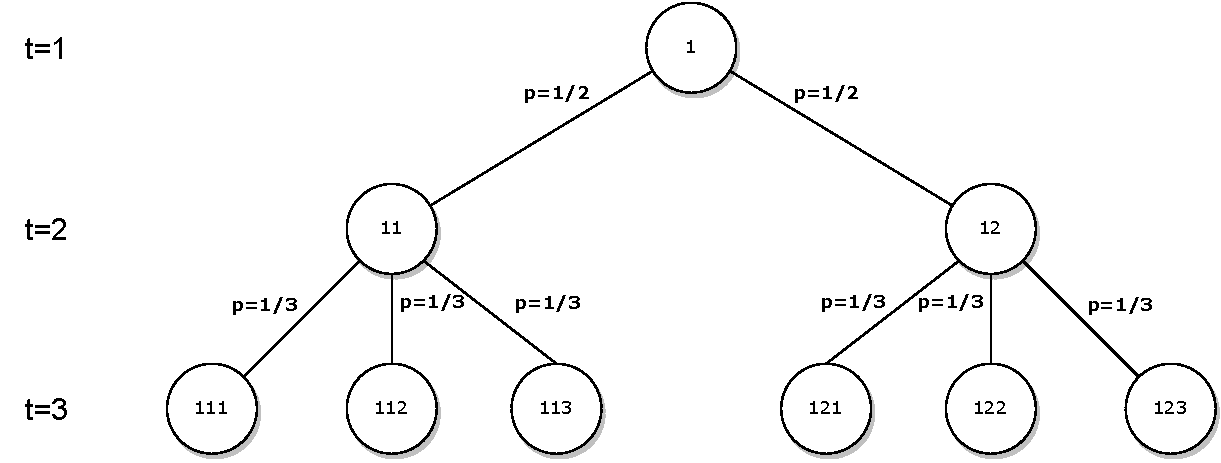
\includegraphics[width=\linewidth]{../img/scenario_tree_balanced.pdf}
  \caption{Balanced scenario tree.}
  \label{fig:balanced_scenario_tree}
\end{figure}


\begin{figure}
  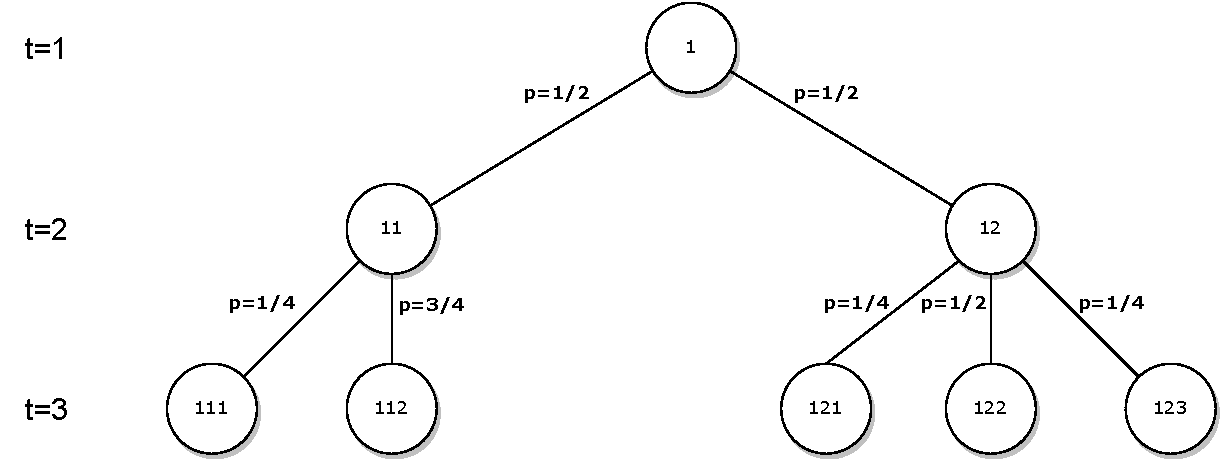
\includegraphics[width=\linewidth]{../img/scenario_tree_unbalanced.pdf}
  \caption{Unbalanced scenario tree.}
  \label{fig:unbalanced_scenario_tree}
\end{figure}

Define \textit{scenario at stage} $t$ as $\xi_{[:t]} = (\xi_1,\dots,\xi_t)$.
Let $S_t(\xi_{[:t-1]})$ be the finite support of the conditional probability distribution of $\xi_t, \, t=3,\dots,T$ and denote $S_2(\xi_{2})$ the finite support of the marginal probability distribution of $\xi_2$. Naturally, we only want to consider sensible scenarios in the set $\mathcal{S}=\{\xi|\xi_t \in S_t(\xi_{[:t-1]}), t=2,\dots,T\}$. Let us now define the probabilities associated with each scenario. Let $P(\xi_{[:T]}^i)$ be the probability of scenario $i$ at the very last stage, i.e.
\begin{equation}
P(\xi_{[:T]}^i)=p_i=P(\xi_2^i)\prod_{t=3}^{T}P(\xi_t^i|\xi_{[:t-1]}), i=1,\dots,S,
\end{equation}
where $S$ (which earlier represented the number of scenarios of a given distribution) now represents the number of scenarios in the very last stage, $P(\xi_2^i)$ is the unconditional marginal probability on $S_2$ in the first stage and $P(\xi_t^i|\xi_{[:t-1]})$ are the conditional probabilities on $S_t(\xi_{[:t-1]})$ in the intermediate stages. The probabilities $P(\xi_2^i)$ and $P(\xi_t^i|\xi_{[:t-1]})$ are termed \textit{arc probabilities} and their products
\begin{equation}
P(\xi_{[:t]}^i)=P(\xi_2^i)\prod_{\tau=3}^{t}P(\xi_\tau^i|\xi_{[:\tau-1]}), i=1,\dots,S, t=3,\dots,T,
\end{equation}
are called \textit{path probabilities}. Obviously, the path probability of scenario $i$ at time $T$ coincides with $p_i$. 	 \todo{We assume that $\xi_1$ is known - make notation consistent! Here we use $P(\xi_1^i)$, which should therefore be $P(\xi_2^i)$}

Two special cases of a scenario tree relevant to this text exist:
\begin{enumerate}
\item Interstage independent tree
	\begin{itemize}
		\item If $P(\xi_t^i|\xi_{[:t-1]})=P(\xi_t^i)$ (the conditional probabilities are equal to the marginal probabilities), then the tree is termed \textit{interstage independent}.
	\end{itemize}
\item Fan of scenarios
\todo{add picture of a fan of scenarios}
	\begin{itemize}
		\item If $S_2(\xi_2)$ and $S_t(\xi_{[:t-1]}), t=3,\dots,T$ are singletons, the tree collapses into a 		\textit{fan of scenarios}.
	\end{itemize}
\end{enumerate}
Having defined the necessary notation for the scenario tree structure, we can now formulate a multistage linear program using a scenario tree. Let $\mathcal{K}_t, t=1,\dots,T$ be disjoint sets of indices enumerating nodes in each stage of the scenario tree ($\mathcal{K}_1=\{1\}$ corresponds to the root node, if the root node has two descendants, then $\mathcal{K}_2=\{2,3\}$ enumerates the descendants and so on).
\newpage
\begin{defn}{Arborescent form of a scenario based linear program \cite[p. 3]{dupacova_scenarios_for_multistage_stochastic_programs}}.
\label{eq:arborescent_linear_programming_formulation}
\footnotesize
\begin{equation}
\mathrm{min} \, c_1^Tx_1 + \sum_{k_2=2}^{K_2}p_{k_2}c_{k_2}^Tx_{k_2} + \sum_{k_3=k_2+1}^{K_3}p_{k_3}c_{k_3}^Tx_{k_3} + \dots +  \sum_{k_T=k_{T-1}+1}^{K_T}p_{k_T}c_{k_T}^Tx_{k_T} \\
\end{equation}
\vspace{-0.5cm}
\begin{alignat}{10}
& s.t. && \, && A_{1,1}x_1 && && \,&&=b_1 \nonumber \\
& && && A_{k_2,1}x_1  + &&A_{k_2,k_2}x_{k_2} && &&=b_{k_2}, k_2 \in \mathcal{K}_2 \nonumber \\
& && && && A_{k_3,a(k_3)}x_{a(k_3)}  + && A_{k_3,k_3}x_{k_3} &&=b_{k_3} , k_3 \in \mathcal{K}_3 \nonumber \\
& && && && && &&  \, \, \, \vdots \nonumber \\
& && && && && A_{k_T,a(k_T)}x_{a(k_T)}  +  A_{k_T,k_T}x_{k_T} &&=b_{k_T} , k_T \in \mathcal{K}_T, \nonumber
\end{alignat}
\vspace{-0.5cm}
\begin{align*}
& l_t \leq x_{k_t} \leq u_t, k_t=K_{t-1}+1,\dots,K_t, \, t=1,\dots,T,  \nonumber
\end{align*}
\normalsize
where $K_1=1$, $\mathcal{K}_t=\{K_{t-1}+1,\dots,K_t\}, \, t=2,\dots,T$, where $a(k_t)$ denotes the predecessor of $k_t$ and where we explicitly set the upper and lower bound ($u_t$ and $k_t$) for the decision variables $x_{k_t}$.
\end{defn}
In definition \ref{eq:arborescent_linear_programming_formulation}, the nonanticipativity constraints are again included implicitly. With the explicit inclusion of nonanticipativity constraints and by taking the expectation over all scenarios, we arrive at a formulation that is more suitable for practical use, see Definition~\ref{eq:scenario_splitted_linear_programming_formulation}. This is the formulation that we will use in the rest of this text as basis for formulating and solving scenario based multistage linear programs.
\begin{defn}
\label{eq:scenario_splitted_linear_programming_formulation}
{Scenario splitted form of a scenario based linear program \\ \cite{defourny_scenario_trees_scenario_splitted_formulation}}.
\footnotesize
\begin{equation*}
\mathrm{min} \, \sum_{i=1}^S p_i \left[ c_1^Tx_1^i + (c_2^i)^Tx_2^i + \dots + (c_T^i)^Tx_T^i  \right]
\end{equation*}
\vspace{-0.5cm}
\begin{alignat}{10}
& s.t. && \, && A_{1,1}x_1 && && \,&&=b_1 \nonumber \\
& && && A_{2,1}^ix_1^i  + &&A_{2,2}^ix_2^i && &&=b_2^i \nonumber \\
& && && && A_{3,2}^ix_{2}^i  + && A_{3,3}^ix_{3}^i &&=b_3^i \nonumber \\
& && && && && &&  \, \, \, \vdots \nonumber \\
& && && && && A_{T,T-1}^ix_{T-1}^i  +  A_{T,T}^ix_{T}^i &&=b_{T}^i, \nonumber
\end{alignat}
\vspace{-0.5cm}
\begin{align}
\label{eq:scenario_splitted_nonanticipativity_constraints}
& i=1,\dots,S \nonumber \\
& l_t \leq x_{t}^i \leq u_t, i=1,\dots,S, \, t=1,\dots,T,  \nonumber \\
& x_t^j=x_t^k, \, \mathrm{if} \, \xi_{[:t]}^j=\xi_{[:t]}^k \, j,k \in \{1,\dots,S\} , t=1,\dots,T,
\end{align}
\normalsize
where Equation \ref{eq:scenario_splitted_nonanticipativity_constraints} represents the nonanticipativity constraints and obviously, the nonanticipativity constraints hold for $t=1$, since $\xi_1$ is deterministic and common to all scenarios.
\todo{define what are quantities $A^i, x^i, c^i, b^i$ under scenario $i$.}
\end{defn}
\subsection{Methods for generation of scenario trees}
There is a plethora of literature on the methods for scenario tree generation. In this section, we aim to present the methods relevant for the purposes of this text in later chapters. Prior to generating a scenario tree, we need to decide the structure of the tree, particularly the number of (decision) stages and the branching structure of the tree (i.e. how many descendants should each node have). This is in general not an easy task, which we will come back to in Section \todo{add reference to curse of dimensionality}.
\subsubsection{Moment matching}
\cite{hoyland_wallace_moment_matching} presented a novel method of generating a scenario tree from historical data that matches some statistical properties of the data, particularly by minimising the distance between moments and correlations calculated from historical data and the moments and correlations calculated from the scenario tree. They formulated a nonlinear optimization program to solve this task. In practical use, this method can be very time demanding and this led to development of a heuristic method for generating scenario trees using moment matching in \cite{hoyland_wallace_moment_matching_heuristic}.  \cite{moment_matching_agarwal} further improved on top of the non-heuristic method and proposed a way to also include empirical cumulative distribution function matching in the program. We will follow the notation established in \cite{moment_matching_agarwal} and describe the optimization program used for generating a simple scenario tree that consists only of a root and $N$ child nodes using the moment matching method.
\begin{rem}
For the purposes of this thesis, we can restrict the theory only to this simple case, as we will be working with stagewise independent balanced scenario trees. Further details on how the moment matching method is used are described in \todo{add reference to chapter where i explain how it all comes together and link specific equation here}. For the more complex case, see \cite{hoyland_wallace_moment_matching}.
\end{rem}
\begin{defn}{Moment matching problem (simple formulation) \cite[p. 9]{moment_matching_agarwal}.}

Let the scenario tree consist of only one stage, i.e. a root and $N$ child nodes. Let $I$ be the set of outcomes to be generated for each scenario, $K$ be the number of moments to be matched, $\mathcal{K}=\{1,\dots,K\}$, $M_{i_k}$ the $k$-th moment calculated from historical data of $i$-th outcome, $C_{i,i'}$ be the correlation calculated from historical data between $i$-th and $i'$-th outcomes. Then the moment matching problem can be formulated as follows:
\begin{alignat}{10}
& && && \sum_{i\in I} \sum_{k\in \mathcal{K}} \left(m_{i,k} - M_{i,k}\right)^2 + \sum_{(i, i') \in I, i < i'}(c_{i,i'}-C_{i,i'})^2 \nonumber \\
& s.t. && \sum_{j=1}^N p_j&&=1 \nonumber \\
& && m_{i,1}&&=\sum_{j=1}^N p_jx_{i,j}, i \in I \nonumber \\
& && m_{i,k}&&=\sum_{j=1}^N p_j(x_{i,j}-m_{i,1})^k, i \in I, k>1 \nonumber \\
& && c_{i,i'}&&=\sum_{j=1}^N(x_{i,j}-m_{i,1})(x_{i',j}-m_{i',1})p_j, i,i' \in I, i<i' \nonumber
\end{alignat}
\vspace{-0.5cm}
\begin{alignat}{10}
& x_{i,j}^L<=x_{i,j}<=x_{i,j}^U, i \in I, j=1,\dots,N, \nonumber \\
& 0 <= p_j <= 1, j=1,\dots,N, \nonumber
\end{alignat}
where $m_{i,k}$ are the moments and $c_{i,i'}$ are the correlations between outcome $i$ and $i'$ calculated from the tree and $p_j$ are the probabilities of each node.
\end{defn}

\todo{Add moment matching method}
\todo{Add my own experience with different solvers}
\todo{Add difference between sequential and whole tree approach, see the citation below}
%Gülpinar N, Rustem G, Settergren R, Simulation and Optimization Ap-
%%proaches to Scenario Generatin, Journal of Economic Dynamics & Control,
%vol. 28, Elsevier Science, 2004 - Moment matching - sequential vs whole tree

\subsubsection{Simulation and clustering}
Another way to generate a scenario tree is to use a parametric model for the underlying process, simulate multiple trajectories of such process and then use a clustering procedure to group similar trajectories in each stage together to obtain a valid scenario tree, see e.g. \cite[Section 3]{dupacova_scenarios_for_multistage_stochastic_programs}. In this section we present the basic theory for Geometric Brownian motion and leave the particulars of clustering to the implementation part of this thesis in \todo{add reference to implementation part where we cover clustering}.
\subsubsection{Geometric Brownian motion}
In this section, we mostly follow \cite[Section 3.2.3.]{glasserman2004monte}. The geometric brownian motion is a fundamental model in asset pricing, its first use in finance dates back to the 1960s and it as been the centerpiece of many groudbreaking models, particularly the Black-Scholes model \cite{black_scholes}. We dive right in to the multivariate case, for the basics, see \cite[Section 3.2.]{glasserman2004monte}.
\begin{defn}{Multidimensional Geometric Brownian motion \cite[p. 104]{glasserman2004monte}.}

A $D$-dimensional random process is called Geometric Brownian motion if it is the solution to the following system of stochastic differential equations:
\begin{equation}
\frac{\mathrm{d} S_i(t)}{S_i(t)}=\mu_i \mathrm{d}t + \sigma_i \mathrm{d}X_t(t), S_i(0)>0, i=1,\dots,D,
\end{equation}
where each $X_i$ is a standard Brownian motion and $\mathrm{corr}(X_i(t),X_j(t))=\rho_{i,j}$. Define matrix $\Sigma$ by its elements as $\Sigma_{i,j}=\sigma_i\sigma_j\rho_{i,j}, i, j = 1,\dots,D$ and $\mu=(\mu_1,\dots,\mu_D)$, then the process $S=(S_1,\dots,S_D)$ is called $D$-dimensional Geometric Brownian motion with drift vector $\mu$ and covariance matrix $\Sigma$, denoted by $S\sim\mathrm{GBM}(\mu, \Sigma)$.
\end{defn}
Using stochastic calculus, an explicit solution to the system of stochastic differential equations can be derived, see Equation \ref{eq:gbm_explicit}.
\begin{equation}
\label{eq:gbm_explicit}
S_i(t)=S_i(0)e^{(\mu_i-\frac{1}{2}\sigma_i^2)t+\sigma_iX_i(t)},i=1,\dots,D.
\end{equation}
\subsubsection{Simulating paths}
Let $A$ be the square root matrix of $\Sigma$, i.e. $\Sigma=AA^T$ (since $\Sigma$ is a covariance matrix, it is positive definite and thus the square root matrix exists and is unique).	 The matrix $A$ is usually obtained by Cholesky decomposition. \cite[Section 3.2.3.]{glasserman2004monte} gives a recurrence relation for simulating the paths of Multidimensional Geometric Brownian motion by using Equation \ref{eq:gbm_recurrence}
\begin{equation}
\label{eq:gbm_recurrence}
S_i(t_{k+1})=S_i(t_k)e^{(\mu_i-\frac{1}{2}\sigma_i^2)(t_{k+1}-t_k)+\sqrt{t_{k+1}-t_k}\sum_{j=1}^DA_{i,j}Z_{k+1,j}},i=1,\dots,D,
\end{equation}
where $Z_k=(Z_{k1},\dots,Z_{kD})\sim N(0,I_D)$ (where $I_D$ is the identity matrix of dimension $D$) and $Z_k$ are independent, $k=1,\dots,N$ and where $t_{i}$ are discrete times such that $0=t_0<t_{i}<t_{i+1}$ for $i=0,\dots,N-1$.
%Kaut M, Wallace SW, Evaluation of Scenario Generation Methods for
%Stochastic Programming, 2003 - Clustering with GBM
\subsection{Curse of dimensionality}
In machine learning in general, the curse of dimensionality is a phenomenon where increasing the complexity (dimension) of a problem leads to much higher (often exponentially higher) computational and memory demands, many times so large that the problem becomes unsolvable. A particularly relevant example is dynamic programming, where all states of a system are (usually recursively) explored to obtain the optimal solution. This means that increasing the dimensionality of the problem exponentially increases the number of states exponentially, leading to a unsolvable problem.

The scenario approach to stochastic optimization suffers from the curse of dimensionality aswell, since the number of scenarios grows with the number of decision stages and the number of descendants in each stage. Many methods have been developed to reduce the number of scenarios (e.g. trimming, reduction, and aggregation methods to obtain trees that are solvable in finite time (we refer the interested reader to \cite[p. 6]{dupacova_scenarios_for_multistage_stochastic_programs})). However, all these methods take the already generated large tree (with predefined branching structure) as input and return a potentially smaller tree that should have similar properties (particularly, the optimal solution of the program based on the smaller tree should not be significantly different than the one obtained by solving the program using the	 larger tree). This may not be the optimal approach, as it is possible that the tree has been made overly large in the first place and a smaller tree would suffice. However, the problem of choosing an optimal scenario tree by choosing the number of stages and branching structure in each stage remains largery unexplored in the literature. \todo{This may not be exactly correct - maybe we should focus more on a large number of time steps and then the other methods fail due to large number of scenarios.}
